\shorthandoff{'}
\begin{markdown*}{%
  hybrid,
  definitionLists,
  footnotes,
  inlineFootnotes,
  hashEnumerators,
  fencedCode,
  citations,
  citationNbsps,
  pipeTables,
  tableCaptions,
}

\chapter{Jaculus-link}

Jaculus-link is a standalone communication library that provides a mechanism for multiplexing multiple channels on a single stream connection and routing multiple channelized connections to a single consumer.

% \section{Features}

%   - multiplexing multiple channels on a single stream connection
%   - routing multiple channelized connections to a single consumer

\section{Architecture}

\subsection{Mux}

The `jac::Mux` class allows the transmission of 256 virtual channels over a single stream connection. The class is a template parametrized by the used protocol. The connection is defined as an object implementing the `Duplex` interface.

The protocol is defined by two types: `Packetizer` and `Serializer`. The `Packetizer` is responsible for decoding the incoming stream into packets, while the `Serializer` is responsible for encoding packets into the stream. The packets then contain the channel ID and the data.

The `Mux` class implements a `ChannelTransmitter` interface, which allows sending data to a specified channel. It can be bound to an object implementing the `ChannelReceiver` interface, which is then used to process the received data.

\subsection{Router}

The `jac::Router` class allows routing packets from different connections to consumers depending on the channel ID and vice versa. The class allows binding `ChannelTransmitter` objects to different IDs and presents a `ChannelReceiver` interface on the same ID used to process the received packets.

On the consumer side, objects implementing `jac::Consumer` interface can be bound to different channel IDs. The `Router` will then route the received packet data, paired with the connection ID, to the appropriate consumer.

\subsection{Communicator}

Different *Communicator* interfaces are used as an abstraction used by the application. The supplied *Communicator* interfaces are:

  - `jac::OutputStreamCommunicator`
  - `jac::BufferedInputStreamCommunicator`
  - `jac::OutputPacketCommunicator`
  - `jac::InputPacketCommunicator`

*PacketCommunicator* types allow the usage of the underlying packetization. They do **not** guarantee any packet capacity, as they map directly to the underlying communication interfaces (e.g., `Mux`), which may use different packet sizes. They are, however, useful for data framing without any additional overhead.

*StreamCommunicator* types, on the contrary, hide the underlying packetization and provide a stream-like interface.

\subsection{Full Jaculus-link pipeline}

The default configuration of the full pipeline provided by the library is shown in the diagram in Figure \ref{fig:link-pipeline}.

\begin{figure}[ht]
    \centering
    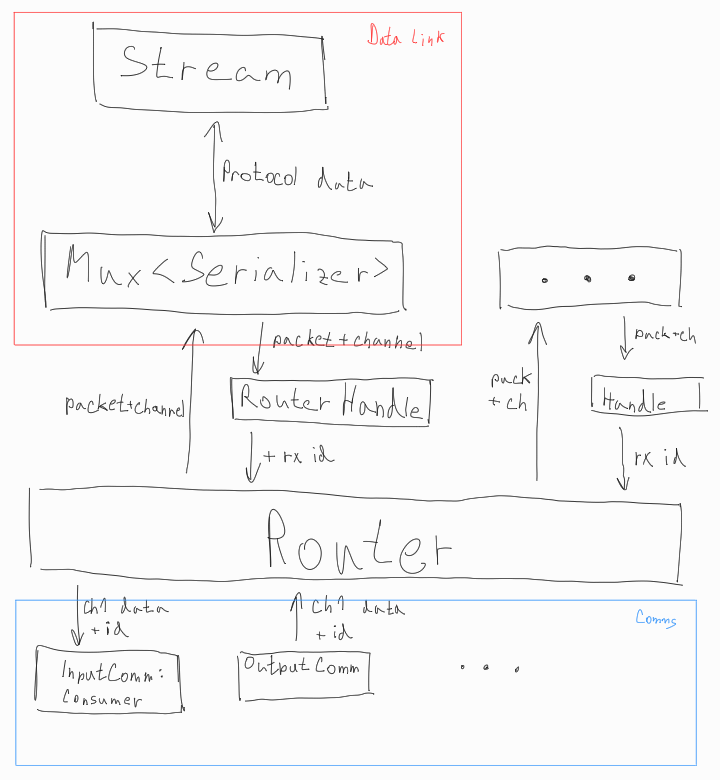
\includegraphics[width=\textwidth]{img/link-pipeline}
    \caption{Default configuration of full Jaculus-link pipeline}
    \label{fig:link-pipeline}
\end{figure}


\section{Implementation}

The library is implemented strictly using only C++ 20 standard library for easy portability. For this reason, no `Duplex` implementation is provided, and the user must provide one themselves.

\subsection{Multiplexer protocol}

The library provides one protocol for the multiplexer in the classes `jac::CobsPacketizer` and `jac::CobsSerializer`. The protocol uses the COBS ((TODO)) algorithm for data framing, which is paired with a CRC16 checksum.  Jaroslav Malec ((TODO)) originally proposed the use of this protocol for the predecessor version of the Jaculus project ((TODO: explain?)). Figure \ref{fig:cobs-diagram} shows a diagram describing the packet structure.

\begin{figure}[ht]
    \centering
    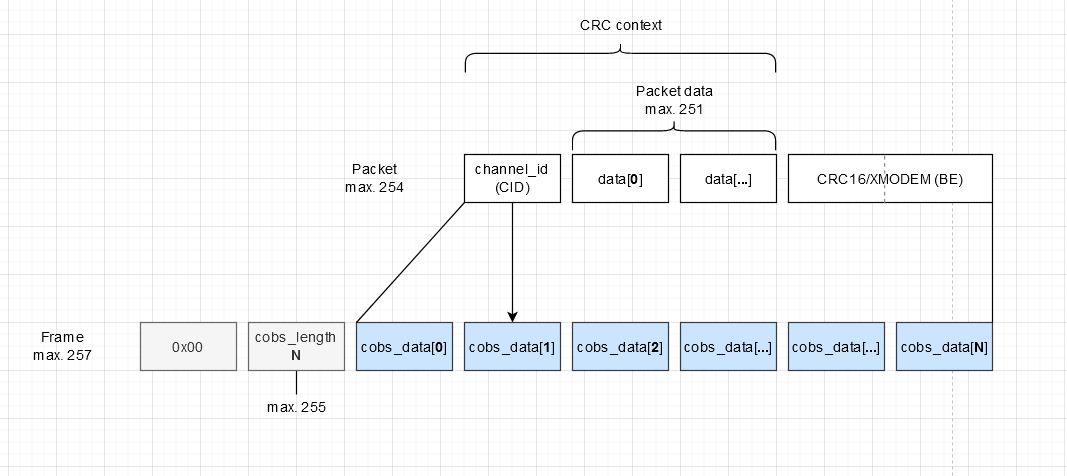
\includegraphics[width=\textwidth]{img/cobs-diagram}
    \caption{COBS protocol packet structure}
    \label{fig:cobs-diagram}
\end{figure}

The delimiter byte at the start of the packet allows for resetting the packetization state in case a packet is lost, malformed, or other corrupted data is received.


\section{Usage}

((TODO: is this even necessary?))

  - defining a Stream
  - configuring Mux
  - configuring Router
  - creating Consumer


\shorthandon{'}
\end{markdown*}